\subsection{Part 5}
% Expected A = -log_10(Experimental T / 100)
% Uncertainty = (1 / (Experimental T * ln(10))) * Uncertainty(Experimental T)
This experiment was performed for three different solutions of blue, green, and red, the results of which are given in Tables \ref{tab:blue}, \ref{tab:green}, and \ref{tab:red} respsectively. The tables include the experimental T and A values, as well as the expected A value calculated using \ref{eq:absorbancce}. The experimental and expected A values agree pretty well; however, for some measurements, these numbers are off by many uncertainties, such as the second measurement in the green dye where the expected A value was $1.733\pm0.00001$, but the experimental A value was $1.848 \pm 0.0005$. These errors exist mainly for small T and large experimental A, so there may be light from other sources interfering with the transmittance measurements to cause this error, since that is more prominent if most of the light is absorbed by the solution.

The absorbance and trasmittances lines for the red light are given in Figure \ref{fig:red_spectrum} (the other lines are given in the Appendix). The colors we observe can easily be explained since the red solution transmitted almost no light in the blue-green range, and transmits lots of light in the red range. Thus, the solution appears red, and this reasoning applies to the blue and green solutions, where the dyes transmit mostly blue and green light respectively and absorb the other wavelengths.

% Blue spectrum

\begin{table}
    \begin{adjustbox}{width=1.1\textwidth, center}
        \begin{tabular}{|c|c|c|c|}
            \hline Experimental T & $1.732 \pm 0.0005$ & $12.213 \pm 0.0005$   & $37.634 \pm 0.0005$     \\
            \hline Experimental A & $1.775 \pm 0.0005$ & $1.042 \pm 0.0005$    & $0.424 \pm 0.0005$      \\
            \hline Expected A     & $1.761 \pm 0.0001$ & $0.91318 \pm 0.00002$ & $0.424420 \pm 0.000006$ \\
            \hline
        \end{tabular}
    \end{adjustbox}
    \caption{Transmittance and Absorbance values for various extrema the solution of blue dye}
    \label{tab:blue}
\end{table}
% Green spectrum

% T: 1.848, 1.496, 3.802, 34.982, 10.416, 10.300, 70.938
% Sorted T: vals = [1.496, 1.848, 3.802, 10.300, 10.416, 34.982, 70.938]
% A: 1.848, 1.928, 1.413, 0.456, 0.983, 0.988, 0.149
% Sorted A (decreasing order): 1.928, 1.848, 1.413, 0.988, 0.983, 0.456, 0.149
\begin{table}
    \begin{adjustbox}{width=1.75\textwidth, center}
        \begin{tabular}{|c|c|c|c|c|c|c|c|}
            \hline Experimental T & $1.496 \pm 0.0005$ & $1.848 \pm 0.0005$ & $3.802 \pm 0.0005$    & $10.300 \pm 0.0005$   & $10.416 \pm 0.0005$   & $34.982 \pm 0.0005$    & $70.938 \pm 0.0005$    \\
            \hline Experimental A & $1.928 \pm 0.0005$ & $1.848 \pm 0.0005$ & $1.413 \pm 0.0005$    & $0.988 \pm 0.0005$    & $0.983 \pm 0.0005$    & $0.456 \pm 0.0005$     & $0.149 \pm 0.0005$     \\
            \hline Expected A     & $1.821 \pm 0.0001$ & $1.733 \pm 0.0001$ & $1.41999 \pm 0.00006$ & $0.98716 \pm 0.00002$ & $0.98230 \pm 0.00002$ & $0.456155 \pm 0.00006$ & $0.149121 \pm 0.00003$ \\
            \hline
        \end{tabular}
    \end{adjustbox}
    \caption{Transmittance and Absorbance values for various extrema the solution of green dye}
    \label{tab:green}
\end{table}

% Red spectrum:
% T: 0.196, 0.080, 1.638, 11.793, 23.230
% Sorted T: vals = [0.080, 0.196, 1.638, 11.793, 23.230]
%A: 2.670, 3.036, 1.793, 0.929, 0.634
% Sorted A (decreasing order): 3.036, 2.670, 1.793, 0.929, 0.634

\begin{table}
    \begin{adjustbox}{width=1.2\textwidth, center}
        \begin{tabular} {|c|c|c|c|c|c|}
            \hline
            Experimental T & $0.080 \pm 0.0005$ & $0.196 \pm 0.0005$ & $1.638 \pm 0.0005$  & $11.793 \pm 0.0005$   & $23.230 \pm 0.0005$     \\
            \hline
            Experimental A & $3.036 \pm 0.0005$ & $2.670 \pm 0.0005$ & $1.793 \pm 0.0005$  & $0.929 \pm 0.0005$    & $0.634 \pm 0.0005$      \\
            \hline
            Expected A     & $3.097 \pm 0.003$  & $2.708 \pm 0.001$  & $1.7857 \pm 0.0001$ & $0.92838 \pm 0.00002$ & $0.633951 \pm 0.000009$ \\
            \hline
        \end{tabular}
    \end{adjustbox}
    \caption{Transmittance and Absorbance values for various extrema the solution of red dye}
    \label{tab:red}
\end{table}

\begin{figure}[H]
    \centering
    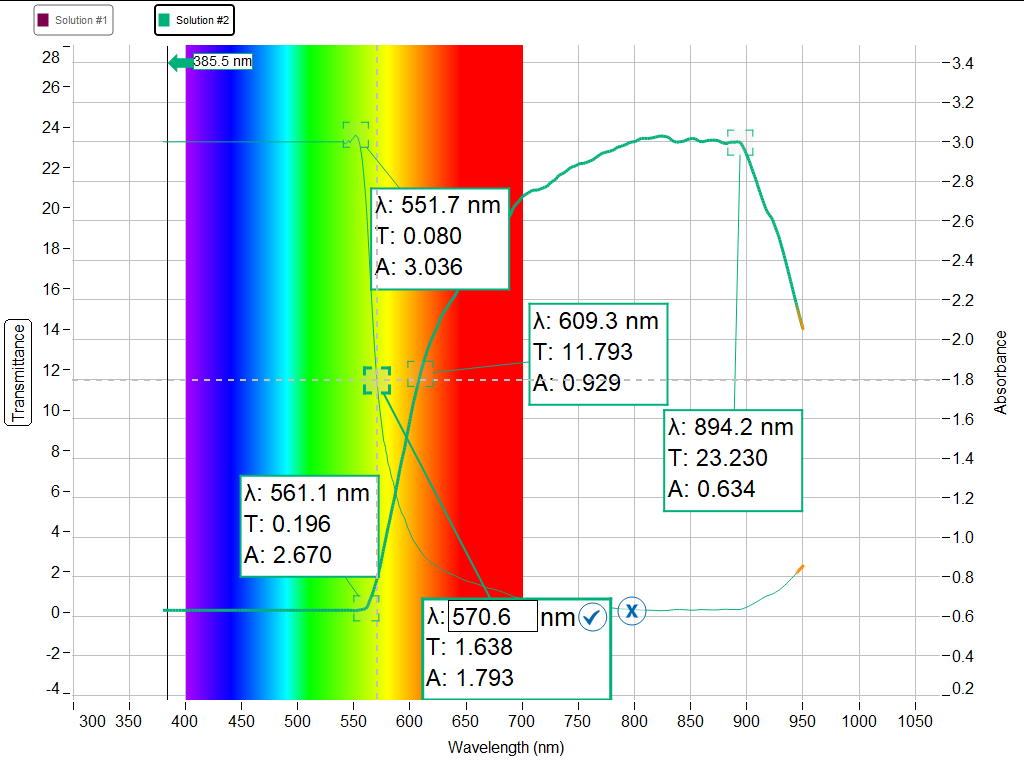
\includegraphics[width=0.8\textwidth]{Results/absorption_spectrometry/red.png}
    \caption{Absorbance and transmittance of red dye}
    \label{fig:red_spectrum}
\end{figure}